\begin{center}
	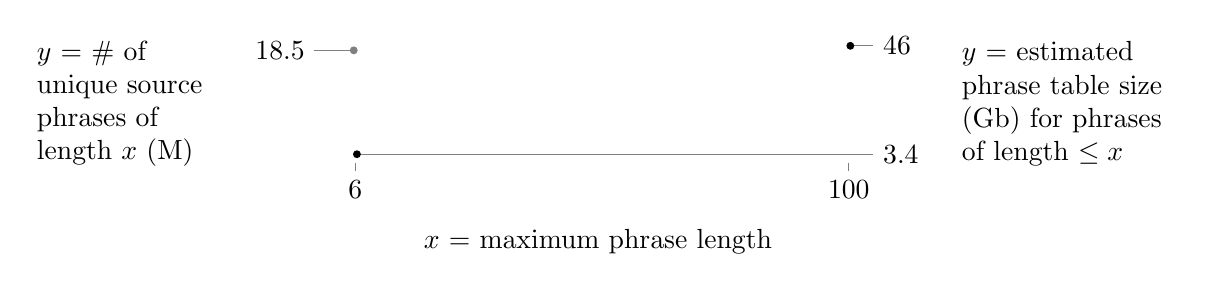
\begin{tikzpicture}[ycomb]
		\node [anchor=east,text width=2.5cm] at (-1,0.75){$y$ = \# of unique source phrases of length $x$ (M)};
		\node [anchor=west,text width=2.7cm]  at (8,0.75) {$y$ = estimated phrase table size (Gb) for phrases of length $\leq x$};

		\draw[gray,thin] (0.42,0.0) -- +(0, -0.1) node [black,anchor=north] {6};
		\draw[gray,thin] (6.68667,0.0) -- +(0, -0.1) node [black,anchor=north] {100};

		\draw[gray,thin] (0.4, 1.42816) -- (-0.1, 1.42816) node [black,anchor=east] {18.5};
		\draw[gray,thin] (0.44, 0.109143) -- (7.0, 0.109143) node [black,anchor=west] {3.4};
		\draw[gray,thin] (6.70667, 1.4858) -- (7.0, 1.4858) node [black,anchor=west] {46};

		\node at (3.5,-1.0) {$x$ = maximum phrase length};
		\draw[gray,thick] plot file {chap-overview/data-ngram-phrases};
		\draw[black,thick] plot file {chap-overview/data-ngram-memory};

		\fill[gray] (0.4, 1.42816) circle (0.05);
		\fill[black] (0.44, 0.109143) circle (0.05);
		\fill[black] (6.70667, 1.4858) circle (0.05);
	\end{tikzpicture}
\end{center}
